\documentclass[UKenglish]{old_el_paso/uiomasterthesis} 
\usepackage{old_el_paso/overhead}
\usepackage{newcommands}

\includeonly{chapters/generation_of_data/data_generation, chapters/cosmological_structure_formation/cosmological_structure_formation}

% Figures
\graphicspath{{/uio/hume/student-u00/johanmkr/Documents/thesis/writing/figures/}} % path to figures

% CHANGE BELOW BETWEEN pdf AND png TO CHANGE QUALITY OF IMAGES

% \def\fileext{pdf} % default file extension for figures
\def\fileext{pdf} % default file extension for figures


% \ifx\fileext\pdf 
%     \def\basepath{main/}
% \else
%     \ifx\fileext\png
%         \def\basepath{temp/} % path to figures
%     % \else
%     %     \def\basepath{}
%     \fi
% \fi 

\newcommand{\basepath}{temp/}
\ifthenelse{\equal{\fileext}{pdf}}{%
    \def\basepath{main/}
}{%
    \ifthenelse{\equal{\fileext}{png}}{%
        \def\basepath{temp/}
    }{%
        \def\basepath{}
    }%
}

\newcommand{\includeimage}[2][]{%
    \includegraphics[#1]{\basepath#2.\fileext}%
}

\title{-sometitle-}        %% ... or whatever
\subtitle{Classifying N-body simulations with and without
relativistic corrections using machine learning
techniques}         %% ... if any
\author{Johan Mylius Kroken}                  %% ... or whoever 

% References
\addbibresource{../references/Project.bib} 
\addbibresource{../references/books.bib}
\addbibresource{../references/ML.bib}
\addbibresource{../references/GR.bib}
% \bibliographystyle{plainnat}
 

\begin{document}
\uiomasterfp[dept={Institute of Theoretical Astrophysics},  %% ... or your department
  program={Computational Science: Astrophysics},                        %% ... or your study program
%   supervisor={The Name},                    %% ... or blank
  supervisors={A David Fonseca Mota\and B Julian Adamek\and C Francisco Antonio Villaescusa Navarro},
  color=green,     %% if more than one
  long]                                     %% ... or short

\frontmatter{}


\begin{abstract}
  
% Background
On large scales, comparable to the horizon, various relativistic effect will affect the observable clustering properties of galaxies. In order to solve for these effects, one need to constantly solve for the metric, velocities and densities in a particular gauge. When simulating large-scale structures we often use N-body simulations, usually performed in the Newtonian limit. However, it is not obvious that Newtonian gravity yield a good global description of an in-homogeneous cosmology when there is significant nonlinear dynamical behaviour ~\parencite{jeong_large-scale_2012}. Literature results suggest that the relativistic corrections necessary on top of realistic Newtonian cosmologies should be very small~\parencite{chisari_connection_2011}. If this is the case, then this justifies the use of Newtonian simulations even on scales larger than the Hubble radius, whose results may be translated into relativistic cosmologies using relevant dictionaries~\parencite{green_newtonian_2012}.

I investigate this by running 2000 simulations with the relativistic N-body code \texttt{gevolution} by~\cite{adamek_gevolution_2016}, with and without relativistic effects, using identical $\Lambda$CDM cosmologies. The simulations are run on a $256^3$ grid each with dimension $5120\text{ Mpc/h}$ in order to capture the Hubble horizon. I investigate the difference between the gravities by considering the power spectra and bispectra of the gravitational potential $\Phi$, the latter should reveal the nonlinear dynamical behaviour present in the relativistic simulation. 

The whole dataset is used to train a Convolutional Neural Network (CNN), aiming to classify the two cases. If successful, the CNN may be used to analyse and understand the features separating the relativistic and Newtonian simulations. This is done through interpretability of the CNN by consider for instance saliency maps ~\parencite{alqaraawi_evaluating_2020} or Grad-CAM~\parencite{selvaraju_grad-cam_2020}. 
\end{abstract}

% \begin{xabstract}[Sammendrag]               %% ... or Abstract or ...
%   Here comes the abstract in a different language.
% \end{xabstract}

\tableofcontents{}                          %%
\listoffigures{}                            %% (omit if none)
\listoftables{}                             %% (omit if none)

\begin{preface}
  Here comes your preface, including acknowledgments and thanks.
\end{preface}

%%%%%%%%%%%%%%%%%%%%%%%%%%%%%%%%%%%%%%%%%%%%%%%%%%%%%%%%%%%%%%%%%%%%%%%%%
%  The main part of the thesis
%%%%%%%%%%%%%%%%%%%%%%%%%%%%%%%%%%%%%%%%%%%%%%%%%%%%%%%%%%%%%%%%%%%%%%%%%

\mainmatter{}

% Introduction
%%%%%%%%%%%%%%%%%%%%%%%%%%%%%%%%%%%%%%%%%%%%%%%%%%%%%%%%%%%%%%%%
%
%   INTRODUCTION
%
%%%%%%%%%%%%%%%%%%%%%%%%%%%%%%%%%%%%%%%%%%%%%%%%%%%%%%%%%%%%%%%%

\chapter{Introduction}\label{ch:introduction}

This is the introduction

\section{Motivation}\label{ch:introduction:motivation}
\section{Outline}\label{ch:introduction:outline}
\section{Aim}\label{ch:introduction:aim}
\section{Nomenclature}\label{ch:introduction:nomenclature}

% PART: Cosmological Structure Formation
%%%%%%%%%%%%%%%%%%%%%%%%%%%%%%%%%%%%%%%%%%%%%%%%%%%%%%%%%%%%%%%%
%
%   COSMOLOGICAL STRUCTURE FORMATION
%
%%%%%%%%%%%%%%%%%%%%%%%%%%%%%%%%%%%%%%%%%%%%%%%%%%%%%%%%%%%%%%%%

\part{Cosmological Structure Formation}\label{part:cosmological_structure_formation}

%   Cosmological Structure Formation
\chapter{Background Cosmology}\label{ch:cosmological_structure_formation:background}
%%%%%%%%%%%%%%%%%%%%%%
%
%   Work related to the theory on cosmological background theory
%
%%%%%%%%%%%%%%%%%%%%%%

\section{The homogeneous Universe}
In this chapter I will focus on explaining the background cosmology in light of a homogeneous universe. A natural place to start is the cosmological principle, followed by a description of the geometry of space itself. If not otherwise stated, the development of this chapter is based on ~\cite{dodelson2020modern}, ~\cite{weinberg2008cosmology} and \TODO{cite Baumann}

\subsection{The Cosmological Principle}



\subsection{The Robertson-Walker Metric}
\begin{equation}
    ds^2 = -dt^2 + a^2(t) \left[ \frac{dr^2}{1-kr^2} + r^2 d\Omega^2 \right]
\end{equation}

\subsection{The Friedmann Equations}



\section{My Universe is loaded with...}

\section{Thermal History of the Universe}

%   Perturbation Theory
\chapter{Perturbation Theory}\label{ch:cosmological_structure_formation:perturbation_theory}
%%%%%%%%%%%%%%%%%%%%%%
%
%   PERTURBATION THEORY
%
%%%%%%%%%%%%%%%%%%%%%%

\section{Initial Conditions}

\section{Transfer Functions}

\section{Power Spectra}

\section{Non-linear Evolution and the Bispectrum}

%   Simulations
\chapter{Simulations}\label{ch:cosmological_structure_formation:simulations}
%%%%%%%%%%%%%%%%%%%%%%
%
%   Work related to the simulation and generation of the dataset
%
%%%%%%%%%%%%%%%%%%%%%%

%% TENSE: past

\section{Parameters}

When performing simulations, it was import to keep all parameters fixed for all the different simulations. The only thing that was changed was the random seed.

    \subsection{Cosmological parameters}
        The relevant cosmological parameters are the dimensionless Hubble factor $h$, the baryon and cold dark matter densities $\Omega_b$ and $\Omega_\mathrm{CDM}$, the Cosmic Microwave Background temperature $T_\mathrm{CMB}$ and the effective number of ultra-relativistic neutrinos $N_\mathrm{ur}$.

        \begin{table}[h]\label{tab:simulations_cosmological_parameters}
            \centering
            \caption{Cosmological parameters}
            \begin{tabular}{c|l|c}
                \toprule
                \textbf{Parameter} & \textbf{Value} & \textbf{Unit} \\
                \midrule
                $h$ & 0.67556 & -\\
                $\Omega_b$ & 0.022032 & -\\
                $\Omega_\mathrm{CDM}$ & 0.12038 & - \\
                $T_\mathrm{CMB} $ & 2.7255 & K \\
                $N_\mathrm{ur}$ & 3.046 & - \\
                \bottomrule
            \end{tabular}
        \end{table}

    \subsection{Primordial power spectrum} 
    The primordial power spectrum, as \TODO{link to when written},contains the pivot scale $k_\mathrm{piv}$, the primordial amplitude, $\mathcal{A}_\mathrm{s}$ and the spectral index, $n_\mathrm{s}$.
        \begin{table}[h]\label{tab:simulations_primordial_parameters}
            \centering
            \caption{Primordial power spectra parameters}
            \begin{tabular}{c|l|c}
                \toprule
                \textbf{Parameter} & \textbf{Value} & \textbf{Unit} \\
                \midrule
                $k_\mathrm{piv}$ & 0.05 & Mpc$^{-1}$ \\
                $\mathcal{A}_\mathrm{s}$ & $2.215\cdot 10^{-9}$ & -\\
                $n_\mathrm{s}$ & 0.9619 & - \\
                \bottomrule
            \end{tabular}
        \end{table}

    \subsection{Box parameters}
    The relevant box parameters were the initial redshift $z_\mathrm{ini}$ where the simulations were started from. The simulations box itself was characterised by the physical length $L$, represented on a cube grid of size $N_\mathrm{grid}^3$, resulting in a resolution of $\Delta_\mathrm{res} = L/N_\mathrm{grid}$. The courant factor \TODO{fill} and time step limit \TODO{fill}.
        \begin{table}[h]\label{tab:simulations_box_parameters}
            \centering
            \caption{Box parameters}
            \begin{tabular}{c|l|c}
                \toprule
                \textbf{Parameter} & \textbf{Value} & \textbf{Unit} \\
                \midrule
                $z_\mathrm{ini}$ & 100 &\\
                $L$ & 5120 & Mpc\\
                $N_\mathrm{grid}$ & 256 & px \\
                $\Delta_\mathrm{res}$ & $20 (=L/N_\mathrm{grid})$ & Mpc px$^{-1}$\\
                Courant factor & 48 & ? \\
                Time step limit & 0.04 & ? \\
                \bottomrule
            \end{tabular}
        \end{table}

    \subsection{Seeds}
        In order to initialise the simulations we used random seeds, one for each simulation. This ensured that analysis performed on different simulations were of different realisations of the simulated universe, essential statistical independence. The seeds, denoted as $\mathtt{S}$ ranged from 0 to 2000, and consisted of the following set:
        \begin{equation}
            \{\mathtt{S} \in \mathbb{Z} | 0 \leq \mathtt{S} < 2000 \}
        \end{equation}

% PART: Machine Learning
%%%%%%%%%%%%%%%%%%%%%%%%%%%%%%%%%%%%%%%%%%%%%%%%%%%%%%%%%%%%%%%%
%
%   DOCUMENT TO BE INCLUDED IN MAIN DOCUMENT AND GOVERN CONTENT RELATED TO THE MACHINE LEARNING CHAPTER
%
%%%%%%%%%%%%%%%%%%%%%%%%%%%%%%%%%%%%%%%%%%%%%%%%%%%%%%%%%%%%%%%%

\part{Machine Learning}\label{part:machine_learning}

\chapter{Fundamental Elements of Machine Learning}\label{ch:machine_learning:fundamental_elements_of_machine_learning}
%%%%%%%%%%%%%%%%%%%%%%%%%%%%%%%%%%%%%%%%%%%%%%%%%%%%%%%%%%%%%%%%
%
%   FUNDAMENTAL ELEMENTS OF MACHINE LEARNING
%
%%%%%%%%%%%%%%%%%%%%%%%%%%%%%%%%%%%%%%%%%%%%%%%%%%%%%%%%%%%%%%%%

\section{Introduction}
In this chapter I will give a brief introduction into machine learning. This includes a mathematical description of some fundamental concepts common across numerous machine learning models. The more advanced models will be dealt with at a later stage. If not otherwise stated, the following chapter is based on ~\cite{Goodfellow-et-al-2016} and ~\cite{hastie2009elements}. 

\section{Linear Algebra}
maybe

\section{Probability and Information Theory}
maybe

\section{Basic Machine Learning}
\TODO{Fill more here}

    \subsection{Estimators, Bias, Variance and Error}

        \paragraph{Estimators} 
        Based on the assumption that there exists some true parameter(s) $\svec{\theta}$ which remain unknown,\footnote{This is the frequentist perspective of statistics} we are able to make predictions and estimations of such parameter(s). Let's say we have $m$ independent and identically distributed (i.i.d.) random variables $\{\vec{x}_1, \vec{x}_2, \dots, \vec{x}_m\}$ drawn from the same probability distribution $p(\vec{x})$. An \textit{estimator} of the true values $\svec{\theta}$ is any function of the data such that $\svec{\hat{\theta}}_m = g(\vec{x}_1,\dots,\vec{x}_m)$, where $\svec{\hat{\theta}}$ is the estimate of $\svec{\theta}$. This is known as point estimation, as we are estimating a single value. This definition does not pose any restrictions on the function $g$. However, a good estimator would yield an estimate $\svec{\hat{\theta}}_m$ that is close to the true value $\svec{\theta}$. 
        
        \paragraph{Function estimators}
        Say we want to predict a variable $\vec{y}$ given some vector $\vec{x}$. We assume the true variable $\vec{y}$ is given by some function approxiamation $f(\vec{x})$ plus some error $\svec{\epsilon}$: $\vec{y} = f(\vec{x}) + \svec{\epsilon}$. The aim is then to estimate the function $f$ with the estimator $\hat{f}$. If we then realise that $\hat{f}$ is really just a point estimator in function space, the two above concepts are equivalent.

        \paragraph{Bias}
        The bias of the estimator $\svec{\hat{\theta}}_m$ is defined as the difference between the expected value of the estimator and the true value of the parameter: $\text{bias}(\svec{\hat{\theta}}_m) = \EE{\estm} - \svec{\theta}$. An unbiased estimator has zero bias, i.e. $\EE{\estm} = \svec{\theta}$. An estimator is asymptotically unbiased if its bias approaches zero as the number of data points $m$ approaches infinity, i.e. $\lim_{m\to\infty} \EE{\estm} = \svec{\theta}$.

        \paragraph{Variance}

        \paragraph{Standard Error}

        \paragraph{Mean Squared Error}


    \subsection{Maximum Likelihood Estimation}
    \subsection{Bayesian Statistics}
    \subsection{Supervised Learning}
    \subsection{Unsupervised Learning}


\chapter{Neural Networks}\label{ch:machine_learning:neural_networks}
%%%%%%%%%%%%%%%%%%%%%%%%%%%%%%%%%%%%%%%%%%%%%%%%%%%%%%%%%%%%%%%%
%
%   NEURAL NETWORKS
%
%%%%%%%%%%%%%%%%%%%%%%%%%%%%%%%%%%%%%%%%%%%%%%%%%%%%%%%%%%%%%%%%

\section{Forward pass - Prediction}
    \subsection{Computational Graphs}
    In order to understand how information flows through a neural network we must understand computational graphs. These are collection of \textit{nodes} and \textit{edged}, where each node represents an \textit{operation} and each edge represents the numerical values as they flow through the network. Nodes may be simple functions such as addition or multiplication but also take more complex. In the latter case, they can be further divided into their respective component, so that the most fundamental computational graph only consists fundamental operations. 

    For example, we consider the functions $\yv = g(\xv)$ and $\zv = f(\yv)$ such that $\zv = f(g(\xv))$. This can be represented as a computational graph as shown in \cref{fig:ML:NN:comp_graph_example}. The computational graph is read from left to right, where the input $\xv$ is fed into the function $g$ which outputs $\yv$. This $\yv$ is then fed into the function $f$ which outputs $\zv$. The computational graph is a visual representation of the function $f(g(\xv))$.

    \begin{figure}[h!]
        \centering
        \begin{tikzpicture}[node distance=2cm and 1.5cm, main/.style = {draw, circle}]
    % Nodes
    \node (left) {};
    \node[main, right=of left] (g) {$g$};
    \node[main, right=of g] (f) {$f$};
    \node[right=of f] (right) {};
    
    % Edges
    \draw[->] (left) -- (g) node[midway,above] {$\vec{x}$};
    \draw[->] (g) -- (f) node[midway,above] {$\vec{y}$};
    \draw[->] (f) -- (right) node[midway,above] {$\vec{z}$};
    
\end{tikzpicture}
        \caption{Computational graph of a function $\vec{z} = f(g(\xv))$.}
        \label{fig:ML:NN:comp_graph_example}
    \end{figure}


    \subsection{Architecture}
        The simplest architecture of a neural network is the fully connected feed forward (FCNN), which consist of $L$ layers in total, the first being an input layer and the remaining $L-1$ layers are called \textit{hidden layers}, $\vec{h}$. Each hidden layer has an \textit{activation} $\vec{a}$, used as an input to an \textit{activation function}, $g$. Mathematically we may write this architecture as:
        \begin{equation}\label{eq:ML:NN:architecture}
            \begin{split}
                \vec{h}^0 &= \vec{x}^{(i)} \\
                \vec{h}^1 &= g_1(\vec{a}^1) \\
                \vec{h}^2 &= g_2(\vec{a}^2) \\
                \vdots & \\
                \vec{h}^{L} &= g_L(\vec{a}^L),
            \end{split}
        \end{equation}
        where $\vec{h}^L$ and $g_L$ are the output layer and output function respectively. The parameter $L$ governs the depth of the neural network. The result of the output layer is simply called the \textit{output} or \textit{predictor}, and typically denoted as $\pred = \vec{h}^L$. When training, we will have a true value, or label, denoted $\yv$. The difference between the true value and the predicted value is called the \textit{residual} or \textit{error}, denoted $\tilde{\yv} = \yv - \pred$. The goal of training is to minimise the error, or equivalently, maximise the likelihood of the true value.



    \subsection{Activation}
        The activation $\vec{a}^l$ of a layer $l$ is an affine transformation of the output of the previous layer, $\vec{h}^{l-1}$. The intercept of this affine transformation is known as the bias $\vec{b}^l$, \footnote{Must not be confused with the statistical bias of an estimator.} typically used to ensure that no activation becomes zero. The activation takes the form:
        \begin{equation}\label{eq:ML:NN:activation}
            \vec{a}^l = (\vec{W}^{l-1\to l})^\mathrm{T}\vec{h}^{l-1} + \vec{b}^l,
        \end{equation}
        where $\vec{W}^{l-1\to l} \in \mathbb{R}^{\mathrm{dim}_{l-1}\cross\mathrm{dim}_l}$ is the matrix of weights describing the mapping from layer $l-1$ to layer $l$. Each layer $l$ has dimension (or neurons) $\mathrm{dim}_l$ which governs the width of each layer. 

        \begin{figure}[h!]
            \centering
            \begin{tikzpicture}[node distance=2cm and 1.5cm, main/.style = {draw, circle}]
  % Nodes
  \node (h_lminus1) {};
  \node[above=of h_lminus1] (w_lminus1_l) {};
  \node[main, right=of h_lminus1] (matmul) {$\texttt{matmul}$};
  \node[main, right=of matmul] (sum) {$\texttt{sum}$};
  \node[main, right=of sum] (g_l) {$g_l$};
  \node[above=of matmul] (b_l) {};
  \node[right=of g_l] (h_l) {};

  % Edges
  \draw[->] (h_lminus1) -- (matmul) node[midway,above] {$\vec{h}^{l-1}$};
  \draw[->] (w_lminus1_l) -- (matmul) node[midway,right] {$(\vec{W}^{l-1\to l})^\mathrm{T}$};
  \draw[->] (matmul) -- (sum) node[midway,above] {$\vec{u}$};
  \draw[->] (b_l) -- (sum) node[midway,right] {$\vec{b}^l$};
  \draw[->] (sum) -- (g_l) node[midway,above] {$\vec{a}^l$};
  \draw[->] (g_l) -- (h_l) node[midway,above] {$\vec{h}^l$};

\end{tikzpicture}

            \caption{Computational graph of a hidden layer of a neural network.}
            \label{fig:ML:NN:comp_graph_hl}
        \end{figure}

    \subsection{Full graph and its output}
        \begin{figure}[h!]
            \centering
            \begin{tikzpicture}[node distance=2cm and 1.5cm, main/.style = {draw, circle}]
    % Nodes
    \node (start) {};
    \node[main, right=of start] (act1) {act};
    \node[main, right=of act1] (g1) {$g_1$};
    \node[right=of g1] (firstdot) {$\cdots$};
    \node[main, right=of firstdot] (act2) {act};
    \node[main, right=of act2] (gl) {$g_l$};
    \node[below=of gl] (seconddot) {$\vdots$};
    \node[main, below=of seconddot] (act3) {act};
    \node[main, left=of act3] (gL) {$g_L$};
    \node[main, left=of gL] (loss) {$\mathcal{L}$};
    \node[above=of loss] (pred) {};
    \node[left=of loss] (end) {};

    % Edges
    \draw[->] (start) -- (act1) node[midway,above] {$\vec{x}/\vec{h}^0$};
    \draw[->] (act1) -- (g1) node[midway,above] {$\vec{a}^1$};
    \draw[->] (g1) -- (firstdot) node[midway,above] {$\vec{h}^1$};
    \draw[->] (firstdot) -- (act2) node[midway,above] {$\vec{h}^{l-1}$};
    \draw[->] (act2) -- (gl) node[midway,above] {$\vec{a}^l$};
    \draw[->] (gl) -- (seconddot) node[midway,right] {$\vec{h}^l$};
    \draw[->] (seconddot) -- (act3) node[midway,right] {$\vec{h}^{L-1}$};
    \draw[->] (act3) -- (gL) node[midway,above] {$\vec{a}^L$};
    \draw[->] (gL) -- (loss) node[midway,above] {$\vec{h}^L/\pred$};
    \draw[->] (pred) -- (loss) node[midway, right] {$\vec{y}$};
    \draw[->] (loss) -- (end) node[midway,above] {$\delta$};
\end{tikzpicture}
            \caption{Computational graph of a fully connected feed forward neural network.}
            \label{fig:ML:NN:comp_graph_whole_FFNN}
        \end{figure}
        The full computational graph of a fully connected neural network is shown in \cref{fig:ML:NN:comp_graph_whole_FFNN}. The output of the network is the output of the output layer, $\vec{h}^L$. The output function is typically a probability distribution, such as the softmax function, or a scalar value, such as the sigmoid function. Either way, the output is the prediction of the network, also noted $\pred = \vec{h}^L$. In order to determine the goodness of this output we must compare it with the target value $\yv$. This is done using a \textit{loss function}, $\mathcal{L}(\yv, \pred)$, which is a function of the prediction and the target. The loss function is a measure of how good the prediction is. The goal of training is to minimise the loss function, or equivalently, maximise the likelihood of the target value. We define the loss $\delta=\mathcal{L}(\yv, \pred)$ which is the error of the prediction. The loss is then used to update the weights and biases of the network, which is done using the \textit{backpropagation} algorithm explained in section \TODO{ref this}


    \subsection{Activation functions}
        The activation functions, $g_l$, are what determines the output of each layer $l$. They can be broadly classifies into two types: \textit{saturating activation functions} and \textit{non-saturating activation function}. For saturating activations, $\lim_{\abs{\vec{x}}\to\infty}\abs{\nabla g(\vec{x})} = 0$. 
        \paragraph{Linear}
            The linear activation is as simple as it gets:
            \begin{equation}\label{eq:ML:NN:activation:linear}
                g(\vec{x}) = a\vec{x} + b \quad \mathrm{and} \quad g'(\vec{x}) = a.
            \end{equation}
            This activation is non-saturating. There is however a problem with using linear activations, \TODO{Write about UNIVERSAL APPROXIMATION THEOREM, here or elsewhere}

        \paragraph{Sigmoid}
            The sigmoid function, or the logistic function is defined as: 
            \begin{equation}\label{eq:ML:NN:activation:sigmoid}
                g(\vec{x}) = \sigma(\vec{x}) = \frac{1}{1+\expe{-\vec{x}}} \quad \mathrm{and} \quad g'(\vec{x}) = g(\vec{x})(1-g(\vec{x}))
            \end{equation}


        \paragraph{Hyperbolic tangent}
            The hyperbolic tangent is defined as:
            \begin{equation}\label{eq:ML:NN:activation:tanh}
                g(\vec{x}) = \frac{\expe{\vec{x}}-\expe{-\vec{x}}}{\expe{\vec{x}}+\expe{-\vec{x}}} \quad \mathrm{and} \quad g'(\xv)=1-g(\xv)^2
            \end{equation}

        \paragraph{Rectified linear unit}
            The rectified linear unit, ReLU, is defined as:
            \begin{equation}\label{eq:ML:NN:activation:relu}
                g(\xv) = 
                \begin{cases}
                    0, \quad & \xv < 0 \\
                    \xv, \quad & \xv \geq 0
                \end{cases}
                \quad \mathrm{and} \quad
                g'(\xv) = 
                \begin{cases}
                    0, \quad & \xv < 0 \\
                    1, \quad & \xv \geq 0.
                \end{cases}
            \end{equation}

        \paragraph{(Scaled) Exponential linear unit}
            The exponential linear unit, (S)ELU, is defined as:
            \begin{equation}\label{eq:ML:NN:activation:selu}
                g(\xv) = \lambda
                \begin{cases}
                    \alpha(\expe{\xv}-1), \quad & \xv < 0 \\
                    \xv, \quad & \xv \geq 0
                \end{cases}
                \quad \mathrm{and} \quad
                g'(\xv) = \lambda
                \begin{cases}
                    \alpha\expe{\xv}, \quad & \xv < 0 \\
                    1, \quad & \xv \geq 0.
                \end{cases}
            \end{equation}
            This function requires two hyperparameters $\alpha$ and $\lambda$.

        \paragraph{Parametric rectified linear unit}
            The parametric rectified linear unit, PReLU, is defined as:
            \begin{equation}\label{eq:ML:NN:activation:prelu}
                g(\xv) = 
                \begin{cases}
                    \alpha \xv, \quad & \xv<0 \\
                    \xv, \quad & \xv\geq 0
                \end{cases}
                \quad \mathrm{and} \quad
                q'(\xv) = 
                \begin{cases}
                    \alpha, \quad & \xv<0 \\
                    1, \quad & \xv\geq 0.
                \end{cases}
            \end{equation}
            If $\alpha=0.01$ this function is also known as the leaky rectified unit, or Leaky ReLU. 

        \paragraph{Softmax}
            The softmax activation function is defined as:
            \begin{equation}\label{eq:ML:NN:activation:softmax}
                g(\xv) = \frac{\expe{\xv}}{\sum_{i=1}^n\expe{x_i}} \quad \mathrm{and} \quad g'(\xv) = g(\xv)(1-g(\xv)).
            \end{equation}
            This activation function is typically used for the output layer of a neural network, where the output is a probability distribution over $n$ classes, i.e. multiclass classification problems. 
    
    \subsection{Loss functions}
        \TODO{write about loss functions}
        \paragraph{MSE}
            \begin{equation}\label{eq:ML:NN:loss:MSE}
                \mathcal{L}_\mathrm{MSE}(\yv, \pred) = \frac{1}{n}\sum_{i=1}^n(y_i-\hat{y}_i)^2 = \frac{1}{n}\tilde{\yv}^\mathtt{T}\tilde{\yv},
            \end{equation}
            where $\tilde{\yv} \equiv \yv-\pred$



        \paragraph{Cross entropy}
            \begin{equation}\label{eq:ML:NN:loss:cross_entropy}
                \mathcal{L}_\mathrm{CE}(\yv, \pred) = -\sum_{i=1}^n y_i\log(\hat{y}_i)
            \end{equation}
            where $\hat{y}_i$ is the predicted probability of class $i$ and $y_i$ is the true probability of class $i$, i.e. the target probability for that class. $n$ is the number of classes. In the binary case, $n=2$, this is equivalent to the binary cross entropy:
            \begin{equation}\label{eq:ML:NN:loss:binary_cross_entropy}
                \mathcal{L}_\mathrm{BCE}(\yv, \pred) = -y\log(\hat{y}) - (1-y)\log(1-\hat{y}).
            \end{equation}

    \subsection{Regularization} % May belongs to forwards pass
            % \TODO{Add dropout, batch normalization, weight decay, early stopping, data augmentation, etc.}

%
%   BACKPROPAGATION
%
\section{Backpropagation - Training}
    \subsection{Chain rule}
        \paragraph{Basics}
        Lets say we have a function $f(x)$ that is composed of two functions $g(x)$ and $h(x)$, such that $f(x) = g(h(x))$. The chain rule states that the derivative of $f(x)$ with respect to $x$ is the product of the derivative of $g(x)$ with respect to $h(x)$ and the derivative of $h(x)$ with respect to $x$:
        \begin{equation}
            \frac{df}{dx} = \frac{dg}{dh} \frac{dh}{dx}.
        \end{equation}
        This can be generalised into the vector case where $f(\vec{x}) = g(h(\vec{x}))$ and $\vec{x} \in \mathbb{R}^n$ and \TODO{write more ahaha}

    \subsection{Backpropagation algorithm}
        The learnable parameters of a neural network are the weights and biases of each layer. In order to update these in an educated\footnote{Instead of just wildly guessing} way, we need to know how the loss, $\delta$, changes with respect to each parameter, $\nabla_{\vec{b}^l}\delta$, $\nabla_{\vec{W}^{l-1\to l}}\delta \quad \forall \; l \in [1,L]$ . This is done using the chain rule, starting from the output layers and working our way backwards through the network. Recalling that the activation is written as \cref{eq:ML:NN:activation} it makes sense to find the derivative of the loss with respect to the output activation:
        \begin{equation}
            \dv{\delta}{a^L_i} = \sum_j\pdv{\delta}{h^L_j}\dv{h^L_j}{a^L_i} = \sum_j\pdv{\delta}{\hat{y}_j}\dv{g_L}{a^L_i}\bigg|_{a^L_j} \leftrightarrow \nabla_{\vec{a}^L}\delta = \nabla_{\pred}\delta \odot \dv{g_L}{\vec{a}^L}\bigg|_{\vec{a}^L},
        \end{equation}
        where $\odot$ is the \textit{element-wise Hadamard product}. The quantity $\nabla_{\vec{a}^L}\delta$ is the gradient of the loss with respect to the output activation. This is propagated backwards through the network as follows:
        \begin{equation}
            \nabla_{\vec{h}^{l-1}}\delta = \vec{W}^{l-1\to l}\nabla_{\vec{a}^l}\delta \quad \mathrm{and} \quad \nabla_{\vec{a}^{l-1}}\delta = \nabla_{\vec{h}^{l-1}}\delta \odot \dv{g_{l-1}}{\vec{a}^{l-1}}\bigg|_{\vec{a}^{l-1}}.
        \end{equation}
        When we know these loss gradients we can compute the gradient of the weight and biases:
        \begin{equation}
            \nabla_{\vec{W}^{l-1\to l}}\delta = \vec{h}^{l-1}(\nabla_{\vec{a}^l}\delta)^T \quad \mathrm{and} \quad \nabla_{\vec{b}^l}\delta = \nabla_{\vec{a}^l}\delta.
        \end{equation}
        We further define a parameter tuple $\Theta^l \equiv (\vec{W}^{l-1\to l}, \vec{b}^l)$ and a gradient tuple $\nabla_{\Theta^l}\delta \equiv (\nabla_{\vec{W}^{l-1\to l}}\delta, \nabla_{\vec{b}^l}\delta)$. The weight and biases of each layer is then updated as $\Theta^l \leftarrow \mathcal{U}(\Theta^l, \nabla_{\Theta^l}\delta)$, where $\mathcal{U}$ is an update function. This is done for each layer $l$ in the network. The backpropagation algorithm is summarised in \cref{alg:ML:NN:backpropagation}.
        \begin{algorithm}
            \caption{Backpropagation algorithm}
            \label{alg:ML:NN:backpropagation}
            \begin{algorithmic}[1]
                \Require{Loss $\delta$, output activation $\vec{a}^L$, output layer $\vec{h}^L$, weight and bias tuples $\Theta^l \equiv (\vec{W}^{l-1\to l}, \vec{b}^l)$, activation functions $g_l$ and update function $\mathcal{U}$.}
                \Ensure{Updated weight and bias tuples $\Theta^l \equiv (\vec{W}^{l-1\to l}, \vec{b}^l)$.}
                \State $\nabla_{\vec{a}^L}\delta \leftarrow \nabla_{\pred}\delta \odot \dv{g_L}{\vec{a}^L}\bigg|_{\vec{a}^L}$
                \For{$l = L, L-1, \ldots, 1$}
                    \State $\nabla_{\vec{h}^{l-1}}\delta \leftarrow \vec{W}^{l-1\to l}\nabla_{\vec{a}^l}\delta$
                    \State $\nabla_{\vec{a}^{l-1}}\delta \leftarrow \nabla_{\vec{h}^{l-1}}\delta \odot \dv{g_{l-1}}{\vec{a}^{l-1}}\bigg|_{\vec{a}^{l-1}}$
                    \State $\nabla_{\vec{W}^{l-1\to l}}\delta \leftarrow \vec{h}^{l-1}(\nabla_{\vec{a}^l}\delta)^T$
                    \State $\nabla_{\vec{b}^l}\delta \leftarrow \nabla_{\vec{a}^l}\delta$
                    \State $\Theta^l \leftarrow \mathcal{U}(\Theta^l, \nabla_{\Theta^l}\delta)$
                \EndFor
            \end{algorithmic}
        \end{algorithm}
        \TODO{Revise this algorithm}

    \subsection{Optimization of parameters}
        \paragraph{Gradient descent}
        The ultimate goal is to arrive at some parameters $\Theta$ that minimize the output loss $\delta$. In order to do so, we must update the parameters until this goal is reached. The question is then \textit{how} we should update these parameters. In the most general case, we need to find some $\Delta\Theta$ such that $\Theta \leftarrow \Theta + \Delta\Theta$, where the only condition is that $\Delta\Theta$ yield a new $\Theta$ whose loss decrease. The backbone of this thinking is the \textit{gradient descent} algorithm, which is a first order optimization algorithm. The idea is that since we want to minimize the loss, which is a function of $\Theta$, we should move in the direction of the negative gradient of the loss with respect to $\Theta$. the most naïve implementation of this is to simply advance in the direction of the negative gradient by a step given by the learning rate\footnote{$\gamma$ is also often referred to as the step size} $\gamma$: $\Delta\Theta = -\gamma\nabla_\Theta\delta$. This is known as \textit{batch gradient descent} and is the most basic form of gradient descent. This would leave us with the following update function:
        \begin{equation}\label{eq:ML:NN:gradient_descent:update_function}
            \mathcal{U} =  \Theta - \gamma\nabla_\Theta\delta.
        \end{equation}
        There are several problems with this approach, the most important of them being:
        \begin{itemize}
            \item The learning rate $\gamma$ is constant, which means that the step size is constant. This can lead to the algorithm getting stuck in local minima.
            \item The gradient is computed using the entire dataset, which can be very computationally expensive.
        \end{itemize}
    
        \paragraph{Stochastic gradient descent}
        To our rescue comes stochastic gradient descent (SGD), which solves both of the above issues, by estimating the gradient using only a subset of the data, called a \textit{mini-batch}. This means that the gradient is computed as an average over the mini-batch, which is a good approximation of the true gradient since the gradient of a dataset is statistically an expectation value. This allows us to increase the dataset without increasing the cost of computing the gradients. We may use several such minibatches chosen at random, say $m$ batches. This would yield the following estimate for the gradient:
        \begin{equation}\label{eq:ML:NN:stochastic_gradient_descent:gradient_estimate}
            \nabla_\Theta\delta \approx \frac{1}{m}\sum_{i=1}^m\nabla_\Theta\delta_i,
        \end{equation}
        where $\delta_i$ is the loss from minibatch $i$. This is known as \textit{mini-batch gradient descent}. The update function for SGD is then identical to \cref{eq:ML:NN:gradient_descent:update_function} but with the gradient estimate from \cref{eq:ML:NN:stochastic_gradient_descent:gradient_estimate}. Choosing minibatches at random also greatly reduce the chances of being stuck in a local minimum. 

        \paragraph{Adding momentum} In order to speed up convergence we may add a momentum term, which takes into account the previously found gradients. This is done by adding a momentum term, called the velocity $\vec{v}$, to the update function. We start with some initial velocity, and it is updated as $\vec{v}\leftarrow \alpha\vec{v}-\gamma\nabla_\Theta\delta$, where $\alpha$ is the momentum hyperparameter, which controls the weight of the previous velocity (and thus the previous gradients). This yields simply $\Delta\Theta = \vec{v}$ and the following update function:
        \begin{equation}\label{eq:ML:NN:stochastic_gradient_descent:momentum:update_function}
            \mathcal{U} = \Theta + \vec{v}.
        \end{equation}
        \TODO{Nesterov momentum?}

        \paragraph{Adaptive momentum} 
        One algorithm that adapts the momentum term is the \textit{Adam} algorithm \TODO{ref Kinga and Ba} which uses the first and second moments of the gradient to adapt the momentum term. The first moment is the mean of the gradient and the second moment is the variance of the gradient. 

        The adam algorithm is given as:
        \begin{algorithm}[h!]
            \caption{Adam}
            \label{alg:ML:NN:adam}
            \begin{algorithmic}[1]
                \Require{Learning rate $\gamma$, decay rates $\beta_1$, $\beta_2$ $\in [0,1)$, first moment $\vec{m}=\vec{0}$, second moment $\vec{v}=\vec{0}$, weight decay rate $\epsilon$ (for numerical stability), initial parameters $\Theta_0$, and timestep $t=0$.}
                \While{$\Theta_t$ not converged}
                    \State $t \leftarrow t + 1$ (Update timestep)
                    \State $\vec{g}_t \leftarrow \nabla_{\Theta_{t-1}}\delta$ (Compute gradient at timestep $t$)
                    \State $\vec{m}_t \leftarrow \beta_1\vec{m}_{t-1} + (1-\beta_1)\vec{g}_t$ (Update biased first moment estimate)
                    \State $\vec{v}_t \leftarrow \beta_2\vec{v}_{t-1} + (1-\beta_2)\vec{g}_t\odot\vec{g}$ (Update biased second moment estimate)
                    \State $\hat{\vec{m}}_t \leftarrow \frac{\vec{m}_t}{1-\beta_1^t}$ (Bias-corrected first moment estimate)
                    \State $\hat{\vec{v}}_t \leftarrow \frac{\vec{v}_t}{1-\beta_2^t}$ (Bias-corrected second moment estimate)
                    \State $\Delta\Theta_t = - \gamma\frac{\hat{\vec{m}}_t}{\sqrt{\hat{\vec{v}}_t}+\epsilon}$ (Compute update)
                    \State $\Theta_{t} \leftarrow \Theta_{t-1} +\Delta\Theta_t$ (Update parameters)
                \EndWhile

                \Return $\Theta_t$ (Resulting parameters)
            \end{algorithmic}
        \end{algorithm}
        The hyperparameters $\beta_1$ and $\beta_2$ are typically set to $0.9$ and $0.999$ respectively, and $\epsilon$ is typically set to $10^{-8}$. The learning rate $\gamma$ is typically set to $0.001$. 

        \paragraph{Learning rate schedules?}

        \paragraph{Batch normalization}


    \section{Challenges in optimization}

        \paragraph{Vanishing gradient}
            The vanishing gradient problem is a problem that arises when using saturating activation functions, such as the sigmoid function. The problem is that the gradient of the loss with respect to the weights and biases of the network becomes very small, which means that the weights and biases are not updated. This is a problem because the network is not learning anything. Another cause of vanishing gradients are flat regions of the loss in parameter space which are neither local minima nor global minima. This is a problem because the gradient is zero in these regions, which means that the network is not learning anything. Examples of such points are saddle points and plateaus. 

        \paragraph{Exploding gradient}
            Another issue are cliffs in parameter space, or very steep regions. This is a problem because the gradient is very large in these regions, which means that the network is learning too much. This can lead to the network diverging.

        \paragraph{Local minima}
            Being stuck in a local minimum means that the network appear to converge and learning stops. However, the optimal parameters are not found, and the converged model is not the best one. It is hard to know if the network is stuck in a local minimum or not.

\section{Regularization}
    In order combat some of the challenged posed in the previous section we use regularization. Regularization is a technique used to prevent overfitting, which is when the network learns the training data too well, and thus does not generalize well to unseen data. This is done by adding a penalty term to the loss function, which penalizes large weights and biases. This is done by adding a regularization term to the loss function:

    \subsection{Parameter norm penalties}

    \subsection{Data augmentation}

    \subsection{Early stopping}

    \subsection{Parameter sharing}

    \subsection{Ensemble methods}

    \subsection{Dropout}

    




\chapter{Convolutional Neural Networks}\label{ch:machine_learning:convolutional_neural_networks}
%%%%%%%%%%%%%%%%%%%%%%%%%%%%%%%%%%%%%%%%%%%%%%%%%%%%%%%%%%%%%%%%
%
%   CONVLUTIONAL NEURAL NETWORKS
%
%%%%%%%%%%%%%%%%%%%%%%%%%%%%%%%%%%%%%%%%%%%%%%%%%%%%%%%%%%%%%%%%

\section{Convolution}
    \subsection{Basic definitions}
        Mathematically, convolution is given as:
        \begin{equation}\label{eq:ML:CNN:convolution:basic_defintion}
            s(t) = (x * w)(t) = \int x(a)w(t-a)\d a.
        \end{equation}
        This definition is purely mathematical. For machine learning purposes we refer to the function $x(a)$ as the \textit{input} and $w(t-a)$ as the \textit{kernel}. The output of the convolution is often called the \textit{feature map}. This is easily generalized to higher dimensions. For example, in two dimensions the discrete convolution between an input image $I$ and a kernel $K$ is given as:
        \begin{equation}\label{eq:ML:CNN:convolution:discrete_convolution}
            S(i,j) = (I * K)(i,j) = \sum_m\sum_n I(m,n)K(i-m,j-n).
        \end{equation}
        If we choose to $\textit{flip the kernel}$ relative to the input $I$, the convolution becomes commutative:
        \begin{equation}\label{eq:ML:CNN:convolution:discrete_convolution_commutative}
            S(i,j) = (K * I)(i,j) = \sum_m\sum_n I(i-m,j-n)K(m,n).
        \end{equation}
        The latter is preferred in a machine learning context as there is less variation in the values of $m$ and $n$ because the size of the kernel is often much smaller than the size of the input. However, there is yet another quantity that is often used in machine learning, namely the \textit{cross-correlation}, which is more intuitive in some sense, because the kernel is not flipped. The cross-correlation is given as:
        \begin{equation}\label{eq:ML:CNN:convolution:cross_correlation}
            S(i,j) = (K \star I)(i,j) = \sum_m\sum_n I(i+m,j+n)K(m,n).
        \end{equation}
        Most convolutional layers in machine learning use the cross-correlation. However, it is often referred to as just a convolution without the kernel flip, so this is the convention used further. An example of such a convolution (kernel not flipped) is illustrated in figure \ref{fig:ML:CNN:convolution:convolution_operation_map_example}.

        \begin{figure}[h!]
            \centering
            \begin{tikzpicture}[
    2d-arr/.style={matrix of nodes, row sep=-\pgflinewidth, column sep=-\pgflinewidth, nodes={draw}}
  ]

  \matrix (mtr) [2d-arr] {
  0 & 1 & 1 & |[fill=orange!30]| 1 & |[fill=orange!30]| 0 & |[fill=orange!30]| 0 & 0\\
  0 & 0 & 1 & |[fill=orange!30]| 1 & |[fill=orange!30]| 1 & |[fill=orange!30]| 0 & 0\\
  0 & 0 & 0 & |[fill=orange!30]| 1 & |[fill=orange!30]| 1 & |[fill=orange!30]| 1 & 0\\
  0 & 0 & 0 & 1 & 1 & 0 & 0\\
  0 & 0 & 1 & 1 & 0 & 0 & 0\\
  0 & 1 & 1 & 0 & 0 & 0 & 0\\
  1 & 1 & 0 & 0 & 0 & 0 & 0\\
  };

  \node[below=of mtr-5-4] {$\mathbf I$};

  \node[right=0.2em of mtr] (str) {$*$};

  \matrix (K) [2d-arr, right=0.2em of str, nodes={draw, fill=teal!30}] {
    1 & 0 & 1 \\
    0 & 1 & 0 \\
    1 & 0 & 1 \\
  };
  \node[below=of K-3-2] {$\mathbf K$};

  \node[right=0.2em of K] (eq) {$=$};

  \matrix (ret) [2d-arr, right=0.2em of eq] {
  1 & 4 & 3 & |[fill=blue!80!black!30]| 4 & 1\\
  1 & 2 & 4 & 3 & 3\\
  1 & 2 & 3 & 4 & 1\\
  1 & 3 & 3 & 1 & 1\\
  3 & 3 & 1 & 1 & 0\\
  };
  \node[below=of ret-4-3] {$\mathbf{I * K}$};

  \draw[dashed, teal] (mtr-1-6.north east) -- (K-1-1.north west);
  \draw[dashed, teal] (mtr-3-6.south east) -- (K-3-1.south west);

  \draw[dashed, blue!80!black] (K-1-3.north east) -- (ret-1-4.north west);
  \draw[dashed, blue!80!black] (K-3-3.south east) -- (ret-1-4.south west);

  \foreach \i in {1,2,3} {
      \foreach \j in {4,5,6} {
          \node[font=\tiny, scale=0.6, shift={(-1.2ex,-2ex)}] at (mtr-\i-\j) {$\times \pgfmathparse{int(mod(\i+\j,2))}\pgfmathresult$};
        }
    }

\end{tikzpicture}
            \caption{\TODO{fix this figure to be correct w.r.t. cross-correlation/convolution} Example of a cross-correlation operation, which we will also call a convolution. The input image is given by the matrix $\mathbf I$ and the kernel is given by the matrix $\mathbf K$. The output is given by the matrix $\mathbf{K \star I}$. The dashed lines indicate which elements of the input and kernel are multiplied together to produce the output. The figure is taken from TikZ.net \TODO{fix this citation}}
            \label{fig:ML:CNN:convolution:convolution_operation_map_example}
        \end{figure}
        Whether the kernel is flipped does not play a huge role in a convolutional neural networks, because the kernel is learned by the network. However, it is important to be aware of the difference between the two definitions, because it can lead to confusion when interpreting both the output of the network and the convolutional layers themselves. 

    \subsection{Properties}
        \paragraph{Feature detection}
            Different kernel has the ability to detect different features in the input. For example, different kernels can detect vertical edges, horizontal edges, corners or even more complex features. These kernels may be manually defined, however this defies the basic concepts of machine learning. These kernels are instead learned by the network, analogous to the weight matrices $\vec{W}$ in a fully connected network. Hence, the output of a convolutional operation is a feature map. 

        \paragraph{Sparse interactions}
            The kernels $\vec{K}$ are usually a lot smaller than the input images $\vec{I}$. This means that each element of the kernel is used multiple times when producing the output feature map, which again allows for fewer parameters stored and faster computations. 

        \paragraph{Parameter sharing}
            Exactly what it sounds like, the same parameters are re-used to produce more than one output. The learnable weights are the same for each element of the feature map. This is also a way to reduce the number of parameters stored and the number of computations needed.

        \paragraph{Equivariance}
            Convolutional layers are equivariant to translation. This means that if the input is translated, the output is translated by the same amount. This is a very useful property when dealing with images, because the location of a feature is not important. For example, if we want to detect an edge in an image, it does not matter where in the image the edge is located.
        All of the above properties are related to each other, but their combinations makes convolutional layers in a network very powerful.
\section{New Layers}
    \subsection{Convolutional layers}
        A convolutional layer is just a layer in the neural network that uses the convolution (or rather the cross-correlation) operation rather than just plain matrix multiplication. Both the input and output may consist of several planes or channels. For example, an input image may have three channels, one for each color (RGB). The output of a convolutional layer may also have several channels. This is useful because it allows the network to learn different features in parallel. For example, one channel may learn to detect vertical edges, while another channel may learn to detect horizontal edges. The output of the convolutional layer is then a stack of feature maps, one for each channel. Let's consider convolutions in 2 dimensions, where we have $C_\mathrm{in}$ input channels and $C_\mathrm{out}$ output channels. The convolutional layer is then defined as:
        \begin{equation}
            \vec{S}(N_i, C_{\mathrm{out}_j}) = \mathrm{bias}(C_{\mathrm{out}_j}) + \sum_{k=1}^{C_\mathrm{in}} \vec{K}(C_{\mathrm{out}_j}, k) \star \vec{I}(N_i, k),
        \end{equation}
        where $N_i$ is some batch of the dataset. In the case where we omit the bias for the convolutional layers and only have one input channel, this reduces to the simpler form: 
        \begin{equation}
            \vec{S}(N_i, C_{\mathrm{out}_j}) = \vec{K}(C_{\mathrm{out}_j}) \star \vec{I}(N_i).
        \end{equation} 
        The above equation uses $C_{\mathrm{out}}$ different kernels to produce the same number of feature maps. 

        \TODO{Figures to show kernel size, padding, stride and dilation}

        \paragraph{Kernel size}
            The kernel size is usually chosen to be odd, because this allows for a central pixel. This is not necessary, but it is a common choice. The kernel size is usually chosen to be small, because this allows for more parameters to be stored in the network. However, the kernel size is usually chosen to be large enough to capture the features we want to detect.

        \paragraph{Padding}
            The padding is used to control the size of the output feature maps. If we do not use any padding, the output feature maps will be smaller than the input feature maps. This is because the kernel cannot be centered on the edges of the input feature maps. The padding is usually chosen to be zero padding, which means that the input feature maps are padded with zeros. This is the simplest choice, but there are other choices as well. For example, we may choose to pad the input feature maps with the edge values. This is called \textit{edge padding}. Another choice is to pad the input feature maps with the reflection of the edge values. This is called \textit{reflection padding}. The padding is usually chosen to be symmetric, which means that the same amount of padding is added to each side of the input feature maps. However, this is not necessary. 

        \paragraph{Stride}
            The stride is used to control the size of the output feature maps. If we do not use any stride, the output feature maps will be smaller than the input feature maps. This is because the kernel cannot be centered on the edges of the input feature maps. The stride is usually chosen to be one, which means that the kernel is moved one pixel at a time. However, the stride can be chosen to be larger than one, which means that the kernel is moved several pixels at a time. The stride is usually chosen to be the same in both the horizontal and vertical directions, but this is not necessary.

        \paragraph{Dilation}
            The dilation is used to control the size of the output feature maps. If we do not use any dilation, the output feature maps will be smaller than the input feature maps. This is because the kernel cannot be centered on the edges of the input feature maps. The dilation is usually chosen to be one, which means that the kernel is moved one pixel at a time. However, the dilation can be chosen to be larger than one, which means that the kernel is moved several pixels at a time. The dilation is usually chosen to be the same in both the horizontal and vertical directions, but this is not necessary.

        All of the above would define how convolution should take place, and also control the dimensions of the resulting feature map. If we, along an axis, have an input dimension of $D_\mathrm{in}$, a kernel size of $K$, a padding of $P$, a stride of $S$ and a dilation of $D$, the output dimension, $D_\mathrm{out}$, is given as:
        \begin{equation}
            D_\mathrm{out} = \left\lfloor {\frac{D_\mathrm{in} + 2P-D(K-1)-1}{S}+1} \right\rfloor
        \end{equation}
    \subsection{Pooling layers}
        Pooling is a form of dimensional reduction. It is used to reduce the size of the feature maps. This is useful because it reduces the number of parameters stored and the number of computations needed. Pooling is usually done in the spatial dimensions, but it can also be done in the channel dimension. Pooling often consists of replacing the output of a small region of the feature map with some summary statistics for that region. Examples of summary statistics used may be max pooling, average pooling or $L^2$ pooling. Max pooling is the most common choice. A consequence of pooling is invariance to local translation. Also note that pooling may not have to bee a separate operation. Similar effects of dimension reduction and translation invariance may equally be obtained by choosing kernel size, padding, stride and dilation such that the dimension of the feature map is reduced. 



% PART: Simulation and Data Verification
%%%%%%%%%%%%%%%%%%%%%%%%%%%%%%%%%%%%%%%%%%%%%%%%%%%%%%%%%%%%%%%%
%
%   DOCUMENT TO BE INCLUDED IN MAIN DOCUMENT AND GOVERN CONTENT RELATED TO THE DATA GENERATION CHAPTER
%
%%%%%%%%%%%%%%%%%%%%%%%%%%%%%%%%%%%%%%%%%%%%%%%%%%%%%%%%%%%%%%%%

\part{Acquiring Data and Training Model}\label{part:simulation_and_data_verification}

\chapter{Simulations}\label{ch:simulation_and_verification:simulations}
%%%%%%%%%%%%%%%%%%%%%%
%
%   Work related to the simulation and generation of the dataset
%
%%%%%%%%%%%%%%%%%%%%%%

%% TENSE: past

\section{Parameters}

When performing simulations, it was import to keep all parameters fixed for all the different simulations. The only thing that was changed was the random seed.

    \subsection{Cosmological parameters}
        The relevant cosmological parameters are the dimensionless Hubble factor $h$, the baryon and cold dark matter densities $\Omega_b$ and $\Omega_\mathrm{CDM}$, the Cosmic Microwave Background temperature $T_\mathrm{CMB}$ and the effective number of ultra-relativistic neutrinos $N_\mathrm{ur}$.

        \begin{table}[h]\label{tab:simulations_cosmological_parameters}
            \centering
            \caption{Cosmological parameters}
            \begin{tabular}{c|l|c}
                \toprule
                \textbf{Parameter} & \textbf{Value} & \textbf{Unit} \\
                \midrule
                $h$ & 0.67556 & -\\
                $\Omega_b$ & 0.022032 & -\\
                $\Omega_\mathrm{CDM}$ & 0.12038 & - \\
                $T_\mathrm{CMB} $ & 2.7255 & K \\
                $N_\mathrm{ur}$ & 3.046 & - \\
                \bottomrule
            \end{tabular}
        \end{table}

    \subsection{Primordial power spectrum} 
    The primordial power spectrum, as \TODO{link to when written},contains the pivot scale $k_\mathrm{piv}$, the primordial amplitude, $\mathcal{A}_\mathrm{s}$ and the spectral index, $n_\mathrm{s}$.
        \begin{table}[h]\label{tab:simulations_primordial_parameters}
            \centering
            \caption{Primordial power spectra parameters}
            \begin{tabular}{c|l|c}
                \toprule
                \textbf{Parameter} & \textbf{Value} & \textbf{Unit} \\
                \midrule
                $k_\mathrm{piv}$ & 0.05 & Mpc$^{-1}$ \\
                $\mathcal{A}_\mathrm{s}$ & $2.215\cdot 10^{-9}$ & -\\
                $n_\mathrm{s}$ & 0.9619 & - \\
                \bottomrule
            \end{tabular}
        \end{table}

    \subsection{Box parameters}
    The relevant box parameters were the initial redshift $z_\mathrm{ini}$ where the simulations were started from. The simulations box itself was characterised by the physical length $L$, represented on a cube grid of size $N_\mathrm{grid}^3$, resulting in a resolution of $\Delta_\mathrm{res} = L/N_\mathrm{grid}$. The courant factor \TODO{fill} and time step limit \TODO{fill}.
        \begin{table}[h]\label{tab:simulations_box_parameters}
            \centering
            \caption{Box parameters}
            \begin{tabular}{c|l|c}
                \toprule
                \textbf{Parameter} & \textbf{Value} & \textbf{Unit} \\
                \midrule
                $z_\mathrm{ini}$ & 100 &\\
                $L$ & 5120 & Mpc\\
                $N_\mathrm{grid}$ & 256 & px \\
                $\Delta_\mathrm{res}$ & $20 (=L/N_\mathrm{grid})$ & Mpc px$^{-1}$\\
                Courant factor & 48 & ? \\
                Time step limit & 0.04 & ? \\
                \bottomrule
            \end{tabular}
        \end{table}

    \subsection{Seeds}
        In order to initialise the simulations we used random seeds, one for each simulation. This ensured that analysis performed on different simulations were of different realisations of the simulated universe, essential statistical independence. The seeds, denoted as $\mathtt{S}$ ranged from 0 to 2000, and consisted of the following set:
        \begin{equation}
            \{\mathtt{S} \in \mathbb{Z} | 0 \leq \mathtt{S} < 2000 \}
        \end{equation}

\chapter{Data Verification}\label{ch:simulation_and_verification:data_verification}
%%%%%%%%%%%%%%%%%%%%%%
%
%   Work related to the verification of the datasets
%
%%%%%%%%%%%%%%%%%%%%%%

\section{Slices of Datacubes}

\section{Power spectra from Theory}

\TODO{Provide some camb and class power spectra here. }

\section{Powerspectra from Simulations}
\begin{figure}
    \centering
    % 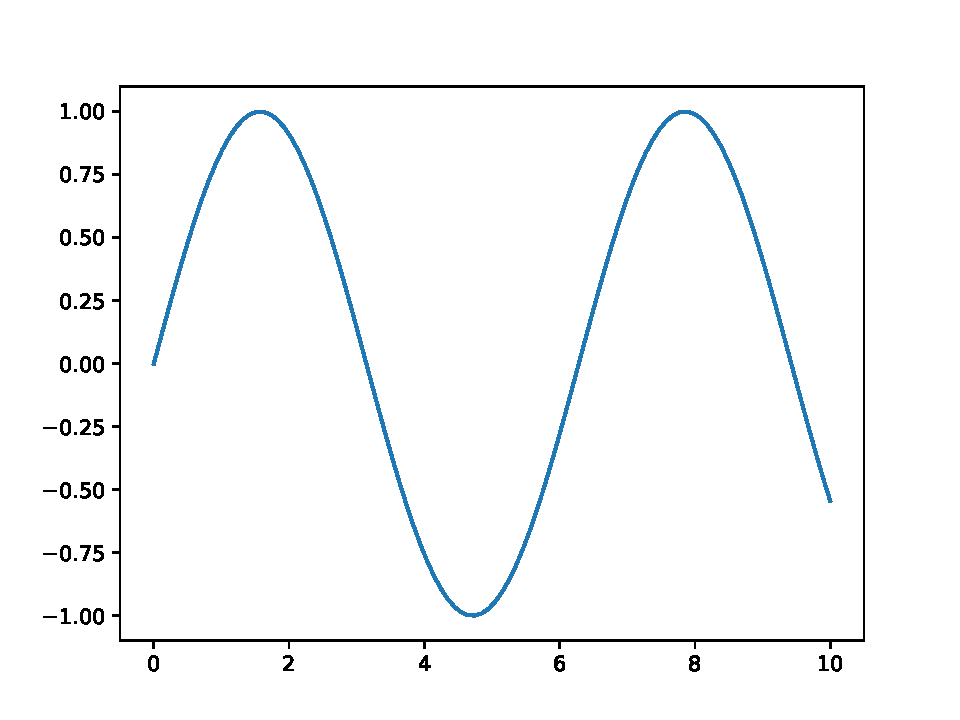
\includegraphics[width=\linewidth]{main/test.pdf}
    \includeimage[width=\linewidth]{nine_matter_power_spectra}
  \end{figure}

  \begin{figure}
    \centering
    % 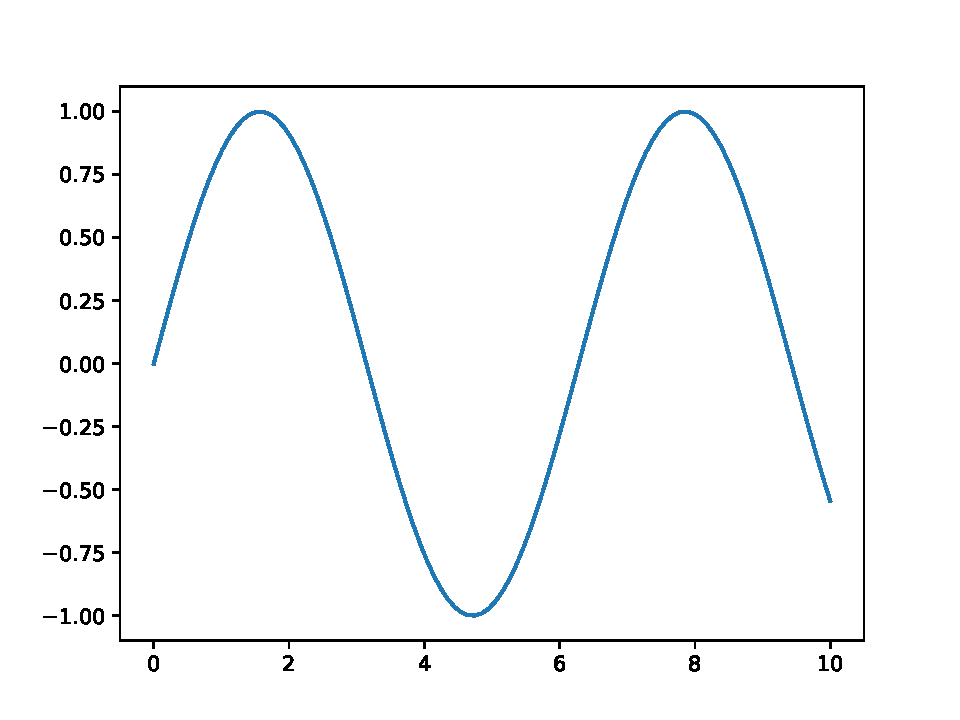
\includegraphics[width=\linewidth]{main/test.pdf}
    \includeimage[width=\linewidth]{average_matter_power_spectrum}
  \end{figure}

\section{Powerspectra from Datacubes}

\section{Analytical Bispectra}

\begin{equation}
  B^{(3)}(k_1,k_2,k_3) = 2\mathcal{P}(k_1)\mathcal{P}(k_2)F_2(\vec{k}_1, \vec{k}_2) + \mathrm{cyc}
\end{equation}

\begin{equation}
  F_2(\vec{k}_1,\vec{k}_2) = \frac{5}{7} + \frac{x}{2}\left(\frac{k_1}{k_2}+\frac{k_2}{k_1}\right) + \frac{2}{7}x^2,
\end{equation}
where $x = \hat{\vec{k}}_1 \cdot \hat{\vec{k}}_2 = \cos{\theta_{12}}$, where $\theta_{12}$ is the angle spanned by $\vec{k}_1$ and $\vec{k}_2$. We could thus consequently write: $F_2(\vec{k}_1,\vec{k_2}) = F_2(k_1,k_2,\theta_{12})$

Given $k_1$ and $k_2$ and $\theta_{12}$ we have the following relations \TODO{Include figure here}:

\begin{equation}
  \begin{split}
    \alpha &= \pi-\theta_{12}\\
    \beta &= \pi-\theta_{23}\\
    \gamma &= \pi-\theta_{31}
  \end{split}
\end{equation}

From cosine rule:
\begin{equation}
  k_3 = \sqrt{k_1^2 + k_2^2 - 2k_1k_2\cos\alpha}
\end{equation}

From the rule of sines \TODO{explain more?}:
\begin{equation}
  \begin{split}
    \beta &= \arcsin\left(\frac{k_1}{k_3}\sin\alpha\right)\\
    \gamma &= \arcsin\left(\frac{k_2}{k_3}\sin\alpha\right)
  \end{split}
\end{equation}

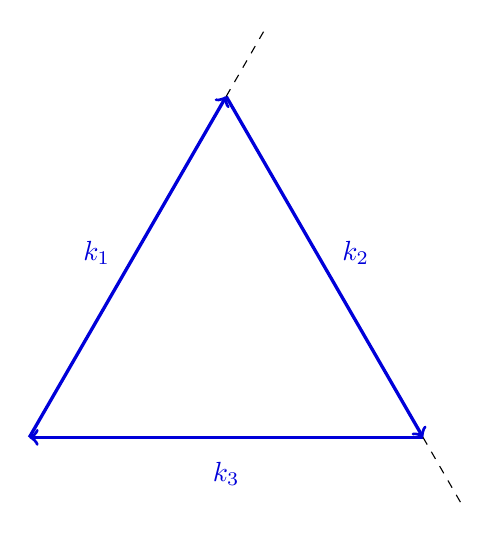
\begin{tikzpicture}
  \colorlet{veccol}{green!70!black}
  \colorlet{vcol}{green!70!black}
  \colorlet{xcol}{blue!85!black}
  \colorlet{projcol}{xcol!60}
  \colorlet{unitcol}{xcol!60!black!85}
  \colorlet{myblue}{blue!70!black}
  \colorlet{myred}{red!90!black}
  \colorlet{mypurple}{blue!50!red!80!black!80}
  \tikzstyle{vector}=[->,very thick,xcol]



  % Define the k vector
  \def\Kone{5}
  \def\Ktwo{5}
  \def\Kthree{5}
  \def\staplelength{1}
  \def\alpha{60}
  \def\beta{60}
  \def\gamma{60}

  \coordinate (k1start) at (0,0);
  \coordinate (k2start) at (\gamma:\Kone);
  \coordinate (k3start) at (\Kthree,0);

  % \Draw vector
  \draw[vector] (k1start) -- (k2start) node[midway, left=20, above=5, right=0] {$\vb{k}_1$};
  \draw[vector] (k2start) -- (k3start) node[midway, right=20, above=5, left=0] {$\vb{k}_2$};
  \draw[vector] (k3start) -- (k1start) node[midway, below=5] {$\vb{k}_3$};
  
  
  % coordinates for the extra stapled lines
  \coordinate (k1staplestop) at ({\Kone*cos(\gamma)+\staplelength*cos(\gamma)}, {\Kone*sin(\gamma)+\staplelength*sin(\gamma)});
  \coordinate (k2staplestop) at ({\Kthree+\staplelength*cos(\beta)}, {-\staplelength*sin(\beta)});

  \draw[dashed] (k2start) -- (k1staplestop);
  \draw[dashed] (k3start) -- (k2staplestop);


  % Template
  % \def\ul{0.52}
  % \def\R{3}
  % \def\ang{60}
  % \coordinate (O) at (0,0);
  % \coordinate (R) at (\ang:\R);
  % \coordinate (X) at ({\R*cos(\ang)},0);
  % \coordinate (Y) at (0,{\R*sin(\ang)});

  % \node[fill=black,circle,inner sep=0.9] (R') at (R) {};
  % \node[above right=-2] at (R') {$(x,y)$};
  % \draw[<->,line width=0.9] %very thick
  %   ({1.2*\R*cos(\ang)},0) -- (O) -- (0,{1.3*\R*sin(\ang)});
  % \draw[projcol,dashed] (X) -- (R);
  % \draw[projcol,dashed] (Y) -- (R);
  % \draw[vector] (O) -- (R') node[midway,left=5,above right=0] {$\vb{r}$};
  % \draw[vector,<->,unitcol]
  %   (\ul,0) node[scale=1,left=2,below left=0] {$\vu{x}$} -- (O) --
  %   (0,\ul) node[scale=1,below=2,below left=0] {$\vu{y}$};
  % \draw pic[->,thick,"$\theta$",draw=black,angle radius=26,angle eccentricity=1.3]
  %   {angle = X--O--R};
  % \draw[thick] (X)++(0,0.1) --++ (0,-0.2) node[scale=0.9,below=-1] {$x = r\cos\theta$};
  % \draw[thick] (Y)++(0.1,0) --++ (-0.2,0) node[scale=0.9,left] {$y = r\sin\theta$};
\end{tikzpicture}

\section{Bispectra from Cube}



\chapter{Trainable Dataset}\label{ch:simulation_and_verification:trainable_dataset}
%%%%%%%%%%%%%%%%%%%%%%
%
%   Work related to the trainable dataset
%
%%%%%%%%%%%%%%%%%%%%%%

\chapter{Machine Learning Model}\label{ch:simulation_and_verification:ml_model}
%%%%%%%%%%%%%%%%%%%%%%
%
%   Work related to the specific machine learning model used
%
%%%%%%%%%%%%%%%%%%%%%%

%% TENSE: past

\section{Framwork}
    % Write about pytorch and why it was chosen

\section{Model Architecture}
    % Write about the model architecture and why it was chosen

\section{Training}
    % Write about the training process and why it was chosen

% \part{Conclusion}                     %% ... or ??
% \chapter{Results}                     %% ... or ??

\backmatter{}

\printbibliography

\end{document}